%
% Documento: Introdução
%

\chapter{Introdução}\label{chap:introducao}

Desde que a Internet foi proposta pelo cientista e pesquisador britânico Tim Bernes-Lee em 1989 \cite{WebHistory}, as páginas \textit{web} vêm mudando de maneira muito acelerada, como pode ser percebido observando os dois gráficos abaixo, gerados com a ajuda do \textit{website} \href{http://httparchive.org/}{HTTP Archieve}. O primeiro gráfico foi gerado com dados de 15 de Abril de 2011 e o segundo com dados de 15 de Abril de 2015, apenas 4 anos de diferença. Os dois mostram a média de dados nas páginas \textit{web} e como esses dados são divididos entre os diferentes tipos de conteúdos que compõe um \textit{website}. Mas o mais impressionante é o dado localizado ao final do gráfico que mostra o tamanho médio de uma página \textit{web} nas respectivas dadas.

\begin{figure}[!htb]
    \centering
    \caption{Média de Bytes por Página por Tipo de Conteúdo em 2011}
    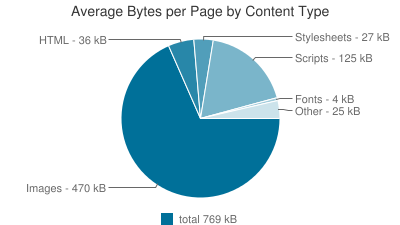
\includegraphics[width=0.3\textwidth]{./04-figuras/introducao/bytes_content_type_april_2011}
    \fonte{\citeonline{HttpArchiveContentType2011}}
    \label{fig:httpcontenttype2011}
\end{figure}

\begin{figure}[!htb]
    \centering
    \caption{Média de Bytes por Página por Tipo de Conteúdo em 2015}
    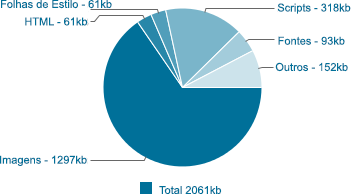
\includegraphics[width=0.3\textwidth]{./04-figuras/introducao/bytes_content_type_april_2015}
    \fonte{\citeonline{HttpArchiveContentType2015}}
    \label{fig:httpcontenttype2015}
\end{figure}

Nos últimos 4 anos o tamanho médio de uma página \textit{web} passou de 769kb para 2061kb, um impressionante aumento de 168\%. Apesar dessa grande mudança no tamanho das páginas (e consequentemente dos \textit{websites}) a maneira como \textit{websites} são entregues do servidor para os clientes não sofreu nenhuma alteração desde 1999, ano de lançamento da RFC 2616 que especificou o HTTP/1.1 \cite{RFC2616}. Como explicado por \cite{Tanenbaum}, o HTTP é um simples protocolo de pedidos e respostas que roda em cima do protocolo TCP. O HTTP ficou famoso por ser fácil de entender e implementar e ao mesmo tempo cumprir sua função com um bom desempenho. Contudo, o aumento do tamanho dos \textit{websites} começou a fazer com que o tempo de resposta das páginas \textit{web} ficasse muito grande, e como mudanças no HTTP não eram possíveis, os desenvolvedores passaram a ter de criar outras formas de resolver esse problema.